\chapter{Data Link Layer}

\section{Introduzione al livello Data Link}

È il layer che si trova a cavallo tra il mondo logico e quello fisico. Fornisce al livello di rete un \textbf{servizio di trasmissione} per flussi di bit (\textbf{bitstream}).

\subsection{Servizi del Data Link Layer}
\begin{itemize}
	\item \textbf{Data framing.}
	\begin{itemize}
		\item Dal basso verso l'alto, dal fisico al logico\\
		raggruppando simboli/bit del layer fisico in frame e \textbf{trasformando il flusso grezzo} di \textbf{bit} in informazioni strutturate. 
		
		\item Dall'alto verso il basso, dal logico al fisico.\\
		incapsulando i datagrammi del livello di rete in frame contenenti due campi, un campo dati $D$ e i campi d'intestazione.
	\end{itemize}
	\begin{figure}[htp]
		\centering
		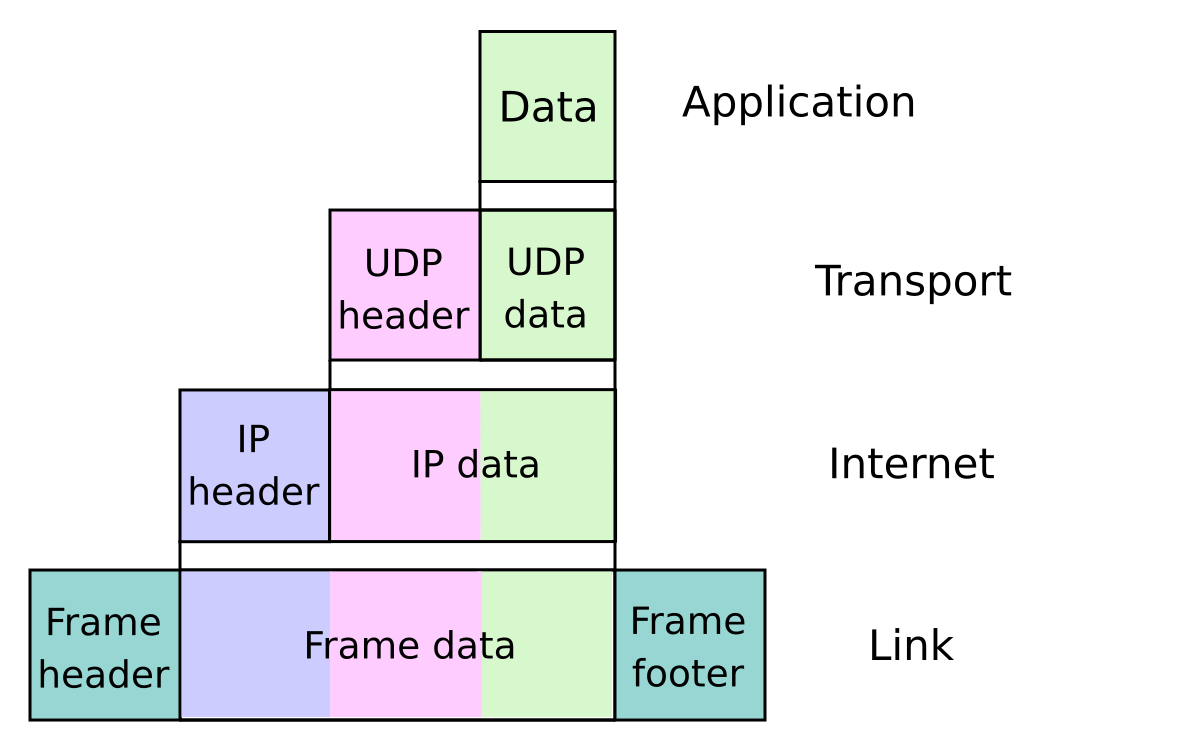
\includegraphics[width=0.5\linewidth]{./images/dataframing.png}
	\end{figure}
	
	\item \textbf{Gestire l'accesso al mezzo fisico}, nel caso di \textbf{canali condivisi}.\\
	I dispositivi, nel DLL, sono identificati tramite indirizzi MAC, dei veri e propri indirizzi fisici. L'accesso al canale condiviso, nel caso dei \textbf{collegamenti broadcast}, dev'essere gestito tramite dei \textbf{protocolli d'accesso multiplo}, per evitare \textbf{collisioni}.
	
	\item Fornire una \textbf{consegna dei dati} \textit{reliable}, \textbf{affidabile}.\\
	Se il mezzo fisico è abbastanza affidabile (fibra, doppino di rame...), non è necessario implementare meccanismi del genere, in quanto ridondanti rispetto a quelli presenti nel livello di trasporto e application. Nel caso di mezzi di trasmissione meno affidabili, come nel caso delle reti wireless, il trasporto reliable è ottenuto tramite meccanismi di ACK/NACK e ritrasmissioni.
	
	\item \textbf{Gestire gli errori} del canale \textbf{di trasmissione} (rilevandoli e, se possibile, correggendoli).\\
	Gli errori possono essere causati da attenuazione del segnale, rumore, interferenze tra campi elettromagnetici o dal mezzo fisico usurato, e sono gestiti tramite checksum, controllo di ridondanza ciclico (CRC), controllo di parità, codici di Hamming o meccanismi simili che conseguono lo stesso scopo.
	
	\item \textbf{Regolare il flusso dati} tra sorgente e destinazione.\\
	I collegamenti possono essere full-duplex o half-duplex, permettendo o non permettendo la trasmissione contemporanea di dati da entrambi i nodi del collegamento. Il pacing di trasmissione deve essere proporzionato a quello di ricezione. I due nodi devono comunicare in maniera opportuna per gestire questa situazione.
\end{itemize}

\subsubsection{Nozione utile - Rumore}
Definiamo come rumore una forma di distorsione (voluta o non voluta) che si presenta all'interno di un segnale elettrico effettivo. Qualsiasi circuito genera rumore, ed è dovuto alla presenza di resistenze (resistenze vere e proprie e resistenza intrinseca dei conduttori elettrici e i materiali usati). Nelle simulazioni dei circuiti elettrici, è possibile inserire un rumore elettrico chiamato \textbf{rumore gaussiano}.

\subsection{Implementazione del DLL - NIC}
In ogni singolo host (device e router) di una rete, è implementato il Data Link Layer. Ciò avviene tramite una combinazione di \textbf{hardware, software e firmware} presente all'interno dei NIC (Network Interface Controller) dei dispositivi di rete. Buona parte del DLL è implementato in hardware, come il protocollo Ethernet nell'adattatore Intel 700, o il protocollo Wi-Fi nel chipset Atheros AR5006. Tuttavia, \textbf{è il software a farsi ponte tra il livello di rete, e il mondo fisico}.

\subsection{Comunicazione tra due Network Interface Controller}
Lato mittente:
\begin{enumerate}
	\item Il datagramma da trasmettere viene incapsulato in un frame del DLL.
	\item I campi d'intestazione del DLL vengono riempiti.
	\item (Se presenti) vengono stabiliti i valori dei bit nei campi per la rilevazione e correzione degli errori.
	\item Il pacchetto viene trasferito.
\end{enumerate}
Dal lato del ricevente:
\begin{enumerate}
	\item Il Network Interface Controller riceve l'intero frame.
	\item (Se presenti) effettua le verifiche relative ai campi di rilevazione e correzione errori.
	\item Estrae il datagramma.
	\item Manda il datagramma al livello di rete+.
\end{enumerate}


\newpage

\section{Data Framing}
Nella trasmissione dei dati, è fondamentale trovare una \textbf{codifica efficace} che permetta di \textbf{interpretare in maniera univoca il segnale elettrico} in stringhe di 0 e 1. A differenza di ciò che si potrebbe pensare, questo problema non è per niente banale. \textbf{Distinguere una sequenza continua di zeri o di 1 da un'interruzione} della trasmissione o da un malfunzionamento \textbf{non è possibile con una codifica a due livelli}.
\begin{figure}[htp]
	\centering
	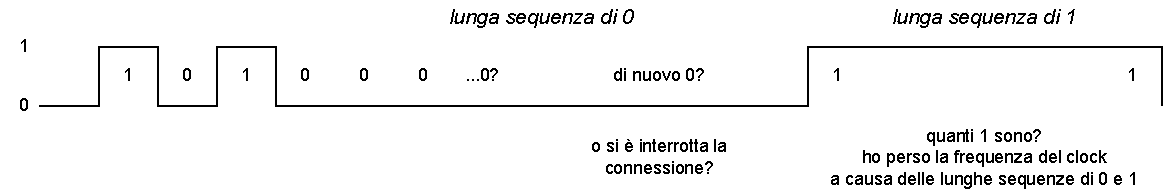
\includegraphics[width=1\linewidth]{./images/2levelencode.pdf}
	\caption{Esempio ipotetico di two-level encoding}
\end{figure}

\subsection{Three-Level Encoding}
Prevede tre livelli di segnale: alto - zero - basso.\\
Segue inoltre delle regole, quali:
\begin{itemize}
	\item Prossimo bit 0.\\
	Nessuna transizione del segnale.
	\item Prossimo bit 1 e livello di segnale $\neq 0$.\\
	Il segnale passa a 0.
	\item Prossimo bit 1 e livello di segnale $=0$.\\
	Il segnale passa ad un livello opposto a quello del più recente segnale diverso da 0.
\end{itemize}

Osserviamo che le transizioni avvengono solo per trasmettere bit $=1$. Inoltre, essendo questa una \textbf{trasmissione asincrona}, una trasmissione di 4 bit$=1$, ossia un ciclo completo, fornirà al receiver un vero e proprio \textbf{clock recovery}, che stabilisce una frequenza di lettura\footnote{Per questo è comune che, in determinati protocolli, la trasmissione sia preceduta da una sequenza di bit chiamata \textbf{preambolo}. Ne parleremo meglio più avanti.} consona, rispetto ai dati in arrivo. 

\begin{figure}[htp]
	\centering
	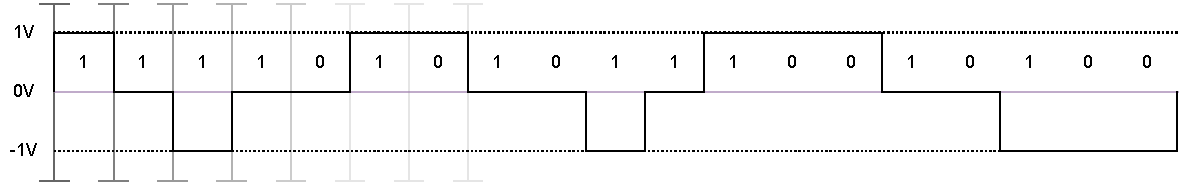
\includegraphics[width=1\linewidth]{./images/3levelencoding.pdf}
\end{figure}

Questo meccanismo di clock permette al receiver di intuire il numero di bit $=0$ da leggere quando, in un quanto di tempo, il segnale rimane ad un certo livello. Chiaramente, lunghe stringhe di zeri possono ancora desincronizzare il receiver, ed è per questo che andremo a parlare (più avanti) di meccanismi che risolvono il problema della \textbf{perdita della sincronizzazione}.


\subsubsection{Esempio di Three-level encoding e Five-level encoding}
\begin{itemize}
	\item La Fast Ethernet (100 BASE TX) utilizza una codifica a tre livelli di segnale: +1V, 0V, -1V. In realtà questi valori non sono statici: sono supportati dei \textbf{range di tollerabilità}.
	\item Specificando più di tre range di voltaggi, e quindi più di tre livelli, diventa possibile trasferire 2 bit alla volta.
	La Gigabit Ethernet (1000 BASE T) utilizza una codifica a cinque livelli: +1V, +0.5V, 0V, -0.5V, -1V. Questa codifica permette di trasmettere in una sola volta i bit \verb|00|, \verb|01|, \verb|10|, \verb|11|, dipendentemente dal livello di segnale.
\end{itemize}

\newpage

\subsection{Codifica a blocchi}
Il three-level encoding è la base per la trasmissione dei dati. Tuttavia, questo meccanismo presenta due criticità:
\begin{itemize}
	\item \textbf{Non è DC-Balanced}. Il livello di tensione medio non è necessariamente mantenuto tendente a 0. Può portare complicazioni di vario tipo.
	\item Se ci sono inoltre lunghe sequenze di zero, si ha un problema di \textbf{perdita di sincronizzazione}.
\end{itemize}
La \textbf{codifica a blocchi} sostituisce blocchi di bit di una determinata dimensione, con blocchi leggermente più grandi ( $4\to5$, $8\to 10$), traducendo le sequenze in maniera tale da garantire un numero minimo di transizioni.

\subsubsection{Codifica 4B5B}
Associa a blocchi di 4 bit, blocchi di 5 bit. Richiede una bandwidth del $25\%$ più capiente. È utilizzata per fast ethernet.

\begin{footnotesize}
	\begin{verbatim}
		Nome    4B           5B          Descrizione
		0       0000         11110       hex data 0
		1       0001         01001       hex data 1
		2       0010         10100       hex data 2
		3       0011         10101       hex data 3
		4       0100         01010       hex data 4
		5       0101         01011       hex data 5
		6       0110         01110       hex data 6
		7       0111         01111       hex data 7
		8       1000         10010       hex data 8
		9       1001         10011       hex data 9
		A       1010         10110       hex data A
		B       1011         10111       hex data B
		C       1100         11010       hex data C
		D       1101         11011       hex data D
		E       1110         11100       hex data E
		F       1111         11101       hex data F
		I       -NONE-       11111       Idle
		J       -NONE-       11000       SSD #1
		K       -NONE-       10001       SSD #2
		T       -NONE-       01101       ESD #1
		R       -NONE-       00111       ESD #2
		H       -NONE-       00100       Halt
	\end{verbatim}
\end{footnotesize}
Questa codifica a blocchi non garantisce DC-balance.
\subsubsection{Codifica 8B10B}

Nella mappatura la sequenza a 8 bit viene divisa in due sottosequenze: una a 5 bit e una a 3 bit. Queste sezioni vengono mappate in modo tale da essere codificate in 6 e 4 bit rispettivamente: concatenate, si ottiene la sequenza di 10 bit. Tra queste sequenze, 12 sono dette \textbf{sequenze di controllo}, come i \textbf{comma}, che permettono al ricevente di allineare in maniera opportuna il flusso di bit. È una codifica \textbf{DC-Balanced}.

\newpage

\subsection{Quantità di informazioni}
Il seguente concetto appartiene alla branca della \textbf{teoria dell'informazione tradizionale}.
Dati $n$ di simboli distinti (in questo caso, livelli di tensione), come \verb|H-M-L| o \\ \verb|HH-HM-HL-MH-MM-ML-LH-LM-LL|, è possibile trasportare un numero di informazioni binarie, quantificate in bit, pari a 
$$
x= \log_2 n
$$


Nel pratico, non potendo esprimere bit parziali, il numero effettivo è dato da

$$
x= \lfloor\log_2 n\rfloor
$$

Con $n=3$ livelli, abbiamo $\lfloor\log_23\rfloor=1$. Con $n=5$ livelli, abbiamo $\lfloor\log_25\rfloor=2$.
Moltiplicando il numero ottenuto, per il numero di step (o simboli) al secondo, otteniamo il \textbf{limite teorico di bitrate}.

$$
\text{Limite teorico bit-rate} = \text{Simboli al secondo} \cdot \log_2 n
$$
\subsubsection{Piccolo approfondimento sulla quantità di informazioni - non è nel programma}
Questa formula è anche detta \textit{Misura di Hartley}, e si tratta di una versione semplificata del concetto di \textbf{entropia informativa di Shannon}, valida solo nel caso di simboli (o eventi) \textbf{equiprobabili}.
\newpage

\section{Gestione degli errori}

\begin{itemize}
	\item L'\textbf{error detection} consiste nell'individuare errori di trasmissione in un frame. Tuttavia non effettua correzione.
	
	\item La \textbf{correzione} permette di individuare errori di trasmissione, ed effettuare correzioni (di dimensioni limitate).
\end{itemize}
Entrambi i metodi sono basati sull'analisi di informazioni ridondanti, per individuare anomalie \\nell'informazione.

\subsection{Ridondanza: elemento di base per l'error detection}
Immaginiamo di voler trasmettere dei dati anagrafici all'interno di un generico pacchetto. Aggiungere allo stesso pacchetto un codice fiscale, mi fornisce delle informazioni sì ridondanti, ma che mi permettono di individuare possibili errori di trasmissione successivamente alla comunicazione.

\subsection{Error Detection}
Un datagramma inoltrato attraverso un mezzo-fisico che ammette errori, contiene al suo interno una sequenza di bit $D$ e un $EDC$ (Error Detection and Correction bits). L'EDC può essere un qualsiasi tipo di controllo, CRC, checksum, controllo di parità.


\begin{figure}[htp]
	\centering
	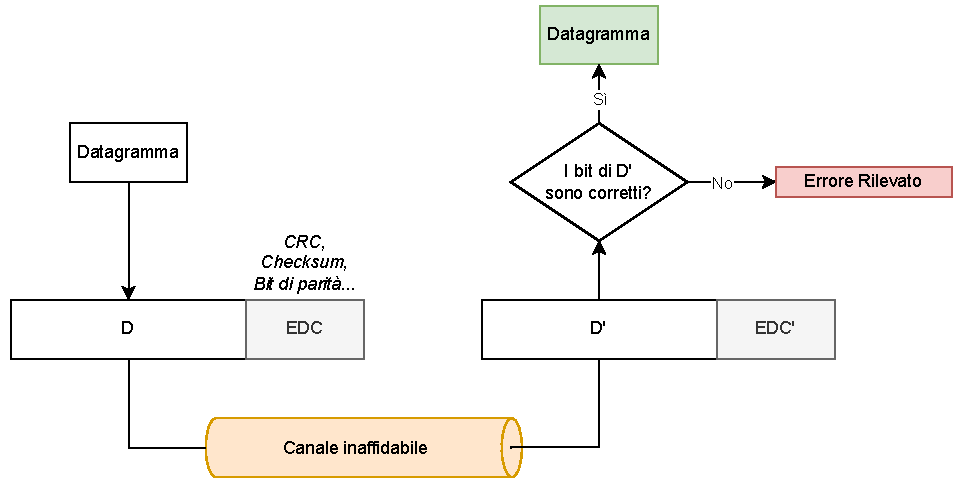
\includegraphics[width=1\linewidth]{./images/edcd.drawio.pdf}
\end{figure}

\newpage


\subsection{Parity check}
Consiste in un bit che specifica se il numero di bit $=1$ è pari o dispari. Può essere un controllo parità a uno o due dimensioni.

\subsubsection{Monodimensionale}
Consente esclusivamente di individuare un errore di trasmissione
\begin{verbatim}
	D:                Parity bit:
	0010011010010101         0      nessun errore rilevato!
	D:                Parity bit:
	0001001010010101         1      nessun errore rilevato!
	D:                Parity bit:
	0010010010010101         0      errore rilevato!
\end{verbatim}
\subsubsection{Bidimensionale}
Consente di individuare e di correggere un errore.
\begin{figure}[htp]
	\centering
	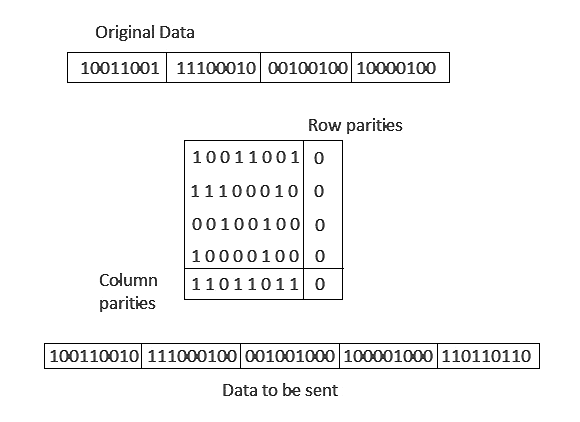
\includegraphics[width=0.75\linewidth]{./images/bidimensionalparitycheck.png}
\end{figure}
\newpage

\subsection{CRC - Cyclic Redundancy Check}
È un metodo di error detection, non correzione. È detto anche controllo dei \textbf{codici polinomiali}. Sfrutta l'aritmetica a $\mod2$, in cui addizione e sottrazione diventano operazioni di $XOR$.

La sequenza di bit $D$ è rappresentata sottoforma di polinomio di grado $d-1=|D|-1$, con coefficienti pari al valore del bit nella sequenza. Il bit più a sinistra è il coefficiente di grado $d-1$ ($x^{d-1}$), quello più a destra è il termine noto ($x^0$). Alla sequenza $D$ \verb|10010111| coinciderà il polinomio:

$$
x^7+ x^4 + x^2 + x^1 + x^0 = x^7+ x^4 + x^2 + x^1 + 1
$$
\begin{itemize}
	\item Sia $D(x)$ il polinomio associato al nostro messaggio $D$.
	\item Sia $G(x)$ il polinomio generatore dello standard di rete. La cifra più significativa è sempre 1.
	\item Sia $r$ il grado di $G(x)$, ed è quindi stabilito dallo standard.
	\item Sia $R(x)=x^r\cdot D(x) \mod G(x)$
\end{itemize}

\subsection{Come effettua il CRC}
Al sender.
\begin{enumerate}
	\item $D$ sono i dati che vogliamo trasmettere.
	\item Calcoliamo $D\cdot 2^r$, nel pratico $D <<r$.
	\item Effettuiamo la divisione $\mod 2$ tra $\frac{D\cdot 2^r}{G}$.
	\item Il resto della nostra divisione sarà il nostro valore di $R$.
	\item Il messaggio che manderemo sarà il risultato della concatenazione di $D+R$. \\In termini di bit: $D\cdot 2^r \ XOR \ \ R$.
	\item Questo valore sarà sempre divisibile per $G$, con resto nullo.
\end{enumerate}

Al receiver.
\begin{enumerate}
	\item Calcola $\frac{\text{Stringa ricevuta}}{G}$.
	\item Se questa divisione ha resto, ci sono stati problemi di trasmissione.
\end{enumerate}

\subsection{Esiti del CRC}
Questo sistema permette di individuare errori a burst al più di $r$ bit. 

\begin{figure}[htp]
	\centering
	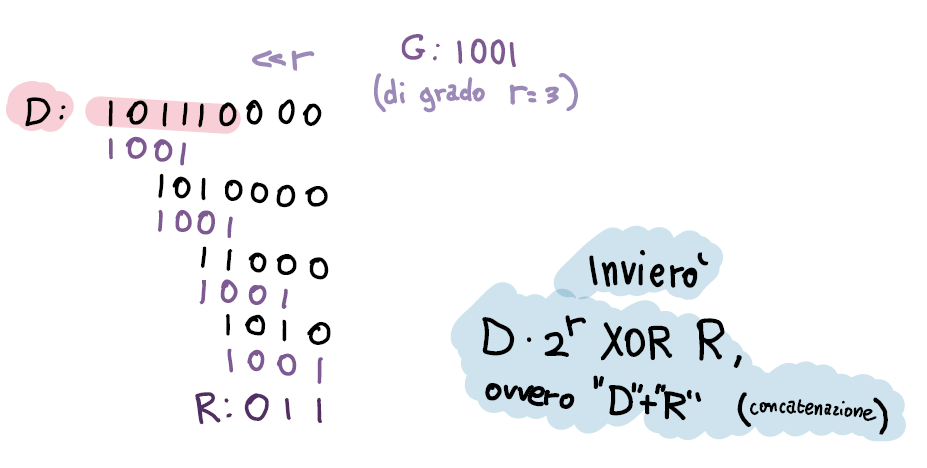
\includegraphics[width=1\linewidth]{./images/crc.png}
\end{figure}

\newpage

\section{Error correction - Perché è difficile?}
Correggere un errore di trasmissione è molto difficile. Il linguaggio naturale gode di contesti (e semantica), tramite cui è possibile estrapolare il significato di una frase, anche quando essa è incompleta!\\ \textit{"Tetto casa rosso" $\to$ "Il tetto della casa è rosso!"}. All'interno di sequenze di bit, non esiste un modo del genere per correggere gli errori. Quello della correzione è un problema molto complesso, verso cui Internet non verte. Quelle di error correction, tuttavia, sono metodologie importanti da conoscere, in quanto utilizzate in molteplici contesti relativi alla trasmissione dati, come all'interno delle RAM.

\subsection{Distanza di Hamming}
Date due codeword, è possibile stabilire una distanza, chiamata \textbf{distanza di Hamming}, che indica il numero di bit che differiscono tra le codeword.
\begin{verbatim}
	10001100 XOR
	11000100  =
	01001000  ->  d=2
\end{verbatim}
Definiamo \textbf{vocabolario} un insieme di codeword. Un vocabolario si dirà \textbf{completo} se, con $n$ bit, avrà $2^n$ codeword.

\subsection{Correzione degli errori - distanza di Hamming}
Limitando un vocabolario a delle stringhe con distanza di Hamming minima fissata, si può ottenere un dizionario del genere:
\begin{figure}[htp]
	\centering
	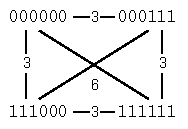
\includegraphics[width=0.5\linewidth]{./images/hamming.pdf}
\end{figure}
con $\min d=3$.\\
Questo limita il numero di stringhe valide, permettendo di introdurre meccanismi di riconoscimento e correzione di errori!
\begin{itemize}
	\item Per \textbf{correggere} $e$ bit di errori, abbiamo bisogno di un vocabolario con distanza minima $d=2e+1$.
	
	
	\item Per \textbf{individuare} $e$ bit di errori, abbiamo bisogno di un vocabolario con distanza minima $d=e+1$.
	
	\begin{figure}[htp]
		\centering
		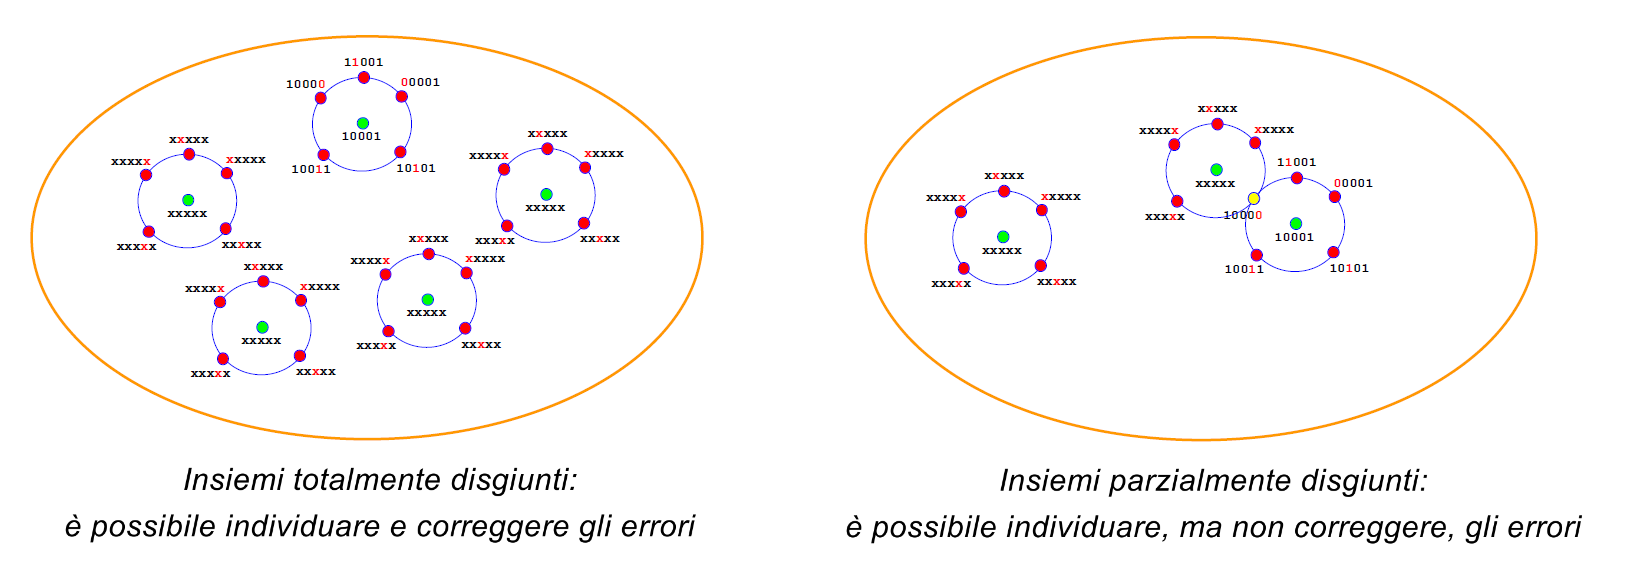
\includegraphics[width=1\linewidth]{./images/correzzioneerrori.png}
	\end{figure}
\end{itemize}

\newpage

\subsection{Dimostrazione distanza minima}
Dato un vocabolario con $m$ bit e $r$ control bit.
$$
m+r = n
$$
Avremo quindi $2^n$ combinazioni, con $2^m$ valide.\\
Data una codeword valida, si ottengono $n$ codeword non valide modificando un singolo bit.

\subsubsection{Formula generale}
$$
\sum _{i=0}^e \binom{m+i}{r} \leq 2^r
$$
Per correggere un errore, avremo:
\begin{footnotesize}
	\begin{verbatim}
		m   r  n  
		1   2  3  
		2   3  5  
		3   3  6  
		4   3  7  
		5   4  9  
		6   4  10 
		7   4  11 
		8   4  12 
		9   4  13 
		10  4  14 
		11  4  15 
		12  5  17 
		
		[...]
	\end{verbatim}
\end{footnotesize}

Per esempio, volessimo trasferire un messaggio di $5$ bit, e volessimo verificare un solo errore $e$, possiamo calcolare:
$$
\sum_{i=0}^{1} \binom{m+i}{r} \leq 2^r
$$
$$
\binom{5}{r} + \binom{6}{r} \leq 2^r
$$
\begin{itemize}
	\item Con $r=0$, $\binom{5}{0} + \binom{6}{0} \leq 2^0 \to 1 + 1 \leq 1 \to 2 \leq 1 $ - falso!
	\item Con $r=1$, $\binom{5}{1} + \binom{6}{1} = \frac{5!}{4!} + \frac{6!}{5!} = \frac{120}{24} + \frac{720}{120} = 5 + 6 = 11 \leq 2^1 $ - falso!
	\item Con $r=2$, $\dots$ - falso
	\item Con $r=3$, $\dots$ - falso
	\item Con $r=4$, $\dots$ - falso
	\item Con $r=5$, $\binom{5}{5} + \binom{6}{5} = 1 + \frac{6!}{5!} = 1 + \frac{720}{120} = 1 + 6 = 7 \leq 2^5 $ - vero!
\end{itemize}

\subsubsection{Reminder utile - formula del coefficiente binomiale}
$$
\binom{n}{k} = \frac{n!}{k!(n-k)!}
$$
\newpage

\subsection{Come si effettua la verifica della distanza di Hamming?}
I bit di controllo sono sempre collocati in posizioni corrispondenti a potenze di due $(1,2,4,8,16,\dots)$.

Il valore del bit di controllo $b_r$ è dato dallo $XOR$ di tutti i valori ottenibili con quel $b_r=1$.\\
Ad esempio, con \verb|xx1x001x0|, abbiamo:
\begin{itemize}
	\item $b_1 = b_3 \ \otimes \ b_5 \ \otimes \ b_7 \ \otimes \ b_9 =  1 \ \otimes \ 0 \ \otimes \ 1 \ \otimes \ 0 = 0$
	\item $b_2 = b_3 \ \otimes \ b_6 \ \otimes \ b_7 = 1 \ \otimes \ 0 \ \otimes \ 1  = 0$
	\item $b_4 = b_5 \ \otimes \ b_6 \ \otimes \ b_7 = 0 \ \otimes \ 0 \ \otimes \ 1  = 1$
	\item $b_8 = b_9 = 0 $
\end{itemize}
E quindi, la stringa che attendiamo, sarà \verb|001100100|.

\subsubsection{Controllo al mittente}
\begin{verbatim}
	001101100
	^^ ^ ! ^
	
	^ = bit da controllare
	| = errore di comunicazione
\end{verbatim}

\begin{itemize}
	\item $b_1 = b_3 \ \otimes \ b_5 \ \otimes \ b_7 \ \otimes \ b_9 =  1 \ \otimes \ 0 \ \otimes \ 1 \ \otimes \ 0 = 0$
	\item $b_2 = b_3 \ \otimes \ b_6 \ \otimes \ b_7 = 1 \ \otimes \ 1 \ \otimes \ 1  = 1$ Errore! Nella stringa ricevuta, $b_2=0$.
	\item $b_4 = b_5 \ \otimes \ b_6 \ \otimes \ b_7 = 0 \ \otimes \ 1 \ \otimes \ 1  = 0$ Errore! Nella stringa ricevuta, $b_3=0$.
	\item $b_8 = b_9 = 0 $
\end{itemize}
L'errore è situato nello slot $b_{2+4} = b_6$. Per correggerlo, effettuiamo un bitflip.
\newpage

\section{Gestire gli accessi multipli}
In una rete, possiamo individuare due tipi di collegamento:
\begin{itemize}
	\item \textbf{Collegamenti punto a punto.}\\
	Sono collegamenti diretti tra trasmittente e ricevente.
	\item \textbf{Collegamenti broadcast.}\\
	Sono collegamenti in cui più nodi trasmittenti e riceventi sfruttano lo stesso canale broadcast.
\end{itemize}

La gestione di un canale broadcast non è un problema per niente intuitivo da risolvere. I protocolli di accesso multiplo gestiscono questo problema, fissando le modalità con cui i nodi regolano le trasmissioni sul canale condiviso.

Quando due nodi cercano di trasmettere sullo stesso canale nello stesso istante, avviene una \textbf{collisione}. Le collisioni causano \textbf{perdite di frame}, e, in eccessiva frequenza, un generale spreco di banda. I \textbf{protocolli di accesso multiplo} gestiscono i canali in maniera consona per non rientrare in situazioni del genere. Esistono tre tipi principali di protocolli per l'accesso multiplo:

\begin{itemize}
	\item \textbf{Protocolli a suddivisione del canale}.\\
	Basati sulla suddivisione del canale in porzioni accessibili esclusivamente ad un nodo.
	\item \textbf{Protocolli ad accesso casuale}.\\
	In cui l'accesso al canale avviene in maniera casuale. Il metodo in questione ammette collisioni, che verranno gestite in maniera opportuna.
	\item \textbf{Protocolli a rotazione - senza collisioni}.\\
	Coordinando opportunamente l’accesso al canale, è possibile evitare le collisioni.
\end{itemize}

\subsection{Protocolli a suddivisione del canale}

\subsubsection{TDMA - Time Division Multiple Access}
Supponiamo una canale broadcast supporti $N$ nodi, e che abbia velocità $R$ bps.\\
TDMA, suddividerà il tempo in \textbf{intervalli di tempo}, e ogni intervallo di tempo in $N$ \textbf{slot temporali}. Ogni slot sarà dedicato ad un nodo: come conseguenza, ogni nodo avrà un tasso di trasmissione di $R/N$ bps. Risolve effettivamente il problema delle collisioni, ma quando si è in uno slot temporale dedicato a un nodo che \textbf{non deve trasmettere nel canale}, avverrà un'attesa non necessaria. 
È un \textbf{protocollo equo}, che \textbf{previene le collisioni}, ma \textbf{limita la banda} di ogni nodo a $R/N$, e porta i nodi in attesa anche quando gli altri non devono trasmettere nulla.

\subsubsection{FDMA - Frequency Division Multiple Access}
Consiste nella suddivisione dello spettro del canale in varie \textbf{bande di frequenza}. A ogni nodo è associata una banda fissa.
Questa suddivisione limita la banda, sempre ad $R/N$, ma non blocca la trasmissione dei nodi.

\subsubsection{CDMA - Code Division Multiple Access}
Consiste nell'associazione di un codice univoco ad ogni nodo. I dati inviati sono codificati secondo quel codice. Con codici opportuni, diventa possibile trasmettere simultaneamente dati a più nodi, e per i nodi, di interpretare in maniera corretta i bit dei dati codificati. Ogni nodo deve conoscere i codici altrui per interpretare correttamente i dati.

\newpage

\subsection{Protocolli ad accesso casuale}
Ogni nodo trasmette alla massima velocità consentita ($R$ bps), e ogni volta che avviene una collisione, i nodi ritrasmetteranno dopo un periodo di tempo casuale (\textit{random delay}). Questo ritardo casuale è indipendente tra i vari nodi, e consente, con buona probabilità, di non subire ulteriori collisioni.\\
\textit{Attenzione, nei seguenti appunti si è deciso di invertire l'ordine con cui, a lezione, sono stati esposti i protocolli ALOHA e Slotted ALOHA. Si è preferito di seguire l'ordine del libro, e di trattare ALOHA come una versione totalmente asincrona di slotted ALOHA}.

\subsubsection{Slotted ALOHA}

\begin{itemize}
	\item Tutti i frame contengono $L$ bit.
	\item Il tempo è suddiviso in slot $L/R$ secondi.
	\item La trasmissione del frame da parte del nodo, inizia all'inizio degli slot.
	\item I nodi sono sincronizzati in modo che tutti sappiano quando iniziano gli slot.
	\item Se in uno slot due o più frame collidono, tutti i nodi della rete rilevano l'evento prima della fine dello slot.
\end{itemize}

Indichiamo $k \in [0,1-K]$, $k, K\in \mathbb{N}$. I nodi slotted ALOHA seguono il seguente comportamento:
\begin{enumerate}
	\item Quando un nodo ha un nuovo frame da spedire, attende l'inizio dello slot successivo, per poi trasmettere il frame.
	
	\item Se non si verifica una collisione, la trasmissione è conclusa.
	
	\item Se si verifica una collisione, il nodo la rileva prima del termine dello slot e ritrasmette il frame dopo $k$ frame, fino a quando l'operazione non ha successo. $k$ è un valore casuale minore di $K$. $K$ cresce ad ogni collisione. 
\end{enumerate}

È un protocollo semplice, che consente ad ogni nodo di lavorare al massimo delle performance possibili, senza limitare i bps a priori. Inoltre, è un protocollo altamente scalabile e abbastanza decentralizzato: l'unica condizione, è che gli slot siano sincronizzati per tutti i nodi.
Tuttavia, ammette collisioni e idle slots, uno spreco generale di slot e un aumento della latenza. 



\subsubsection{Unslotted ALOHA}
È una versione totalmente asincrona dello slotted ALOHA. Il nodo mittente aspetterà un tempo pari al Round Trip Time, in attesa di un ACK. Se l'ACK non arriva, il nodo intuirà che è avvenuta una collisione. In tal caso, aspetterà un quanto di tempo di durata casuale (ma inclusa in un range determinato). Le performance migliori, sono ottenute dalla versione con gli slot temporali.
\begin{figure}[htp]
	\centering
	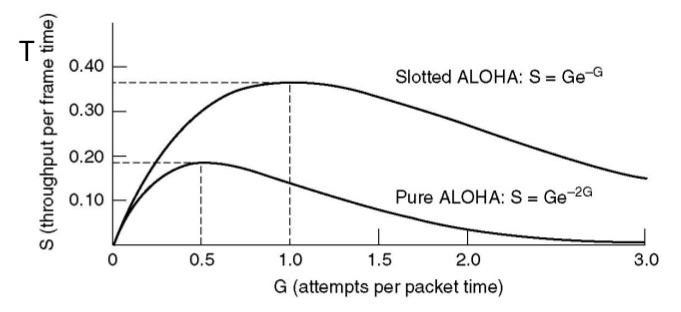
\includegraphics[width=1\linewidth]{./images/ALOHAvsslottedALOHA.png}
\end{figure}

È un grande prezzo da pagare quello per la completa asincronia: l'algoritmo slotted ha un throughput complessivo due volte più grande di quello slotted. L'intuizione è banale: nella versione slotted di ALOHA, due frame possono essere mandati solo all'inizio dello slot temporale. Nella versione unslotted, i frame possono collidere anche a metà trasmissione.

\newpage

\subsubsection{CSMA - Carrier Sense Multiple Access}
I protocolli ALOHA, portano i nodi a decidere di trasmettere indipendentemente dall'attività degli altri nodi. I protocolli CSMA introducono un meccanismo di \textbf{rilevamento della portante} del canale, per "ascoltare" se \textbf{altri nodi stanno già trasmettendo}.
In questo modo, i nodi trasmetteranno esclusivamente quando non rilevano alcuna trasmissione già presente nel canale.\\
Al contrario di ciò che si potrebbe pensare, questo protocollo non sconfigge definitivamente la problematica delle collisioni.
La velocità di trasmissione (nonostante spesso sia altissima) è un fattore non trascurabile.
\begin{enumerate}
	\item Il nodo $A$ trasmette all'istante $t_0$.
	\item $B$ misura la portata del canale all'istante $t_1>t_0$. 
	\item All'istante $t_1$ i bit trasmessi da $A$ potrebbero non essersi propagati fino a $B$.
	\item $B$ trasmette. Collisione!
\end{enumerate}


\subsubsection{CSMA-CD - Carrier Sense Multiple Access con Collision Detection}
Un miglioramento è ottenuto se si introduce un meccanismo di collision detection in aggiunta a quello di rilevamento della portante: la scheda che avrà trasmesso un determinato frame continuerà a misurare il carico del canale. Se rileva rumore o energia di altre trasmissioni nel canale, il nodo interromperà istantaneamente la trasmissione del frame, manderà un \textbf{segnale di jamming con backoff} a tutti gli host, informando tutti i nodi della collisione, e attenderà un quantitativo di tempo casuale per poi ritrasmettere. Questo tempo è chiamato \textbf{tempo di backoff}, non è fissato (intuitivamente renderebbe inutilizzabile il protocollo), e dipende dall'algoritmo scelto dal protocollo.

Un esempio di algoritmo, è quello di \textbf{attesa binaria esponenziale}, o \textit{binary exponential backoff}:
all'$n$-esima collisione, si estrae un valore dall'insieme $K=\{0,1,2,\dots,2^n-1\}$.
Si aspetterà quindi un tempo $T = K \cdot T_\text{slot}$. Il tempo $T_\text{slot}$ dipende dal protocollo: in Ethernet, coincide col tempo richiesto per trasmettere 512 bit, $n$ non supera mai 10, e quindi $0\leq K \leq1023$.

È un ottimo protocollo, ma la collision detection deve avvenire rapidamente: risulta difficile da implementare in reti wireless.

\subsection{Protocolli senza collisioni}
Questi protocolli \textbf{prevengono le collisioni} introducendo dei \textbf{meccanismi preliminari alle trasmissioni}, ottenendo una sincronizzazione consona tra i vari nodi.

\subsubsection{Protocollo bit map - una sorta di prenotazione!}
Con $N$ nodi, il tempo verrà in primis suddiviso in $N$ mini-slot che consentono la trasmissione di un bit. Prima delle trasmissioni effettive, ogni nodo inserirà 1 o 0 nel proprio mini-slot. In questo modo, ogni nodo potrà annunciare se ha intenzione di trasmettere un frame (1) o di non trasmettere (0).
Alla fine di questa trasmissione iniziale, si avrà una \textbf{mappa di bit}, che permetterà ai nodi di seguire un ordine di trasmissione tale da non causare collisioni.

\subsubsection{Binary Backward Counting - una sorta di... torneo?}
In questo protocollo, ogni nodo presenta un ID binario. Questo ID permetterà di risolvere il problema delle collisioni col seguente approccio. Supponiamo $A,B,C,D$ siano dei nodi intenzionati a trasmettere:
\begin{enumerate}
	\item Supponiamo che i nodi $A,B,C,D$ abbiano rispettivamente id \verb|0010|, \verb|1010|, \verb|0100|. \verb|1100|.
	\item Tutti i nodi condividono nel proprio mini-slot, la cifrà più significativa del proprio id.\\
	$A:0$, $B:1$, $C:0$, $D:1$.
	\item Escono dalla competizione i nodi con prima cifra 0. Si passa alla seconda cifra significativa.
	\item $B:0$ $D:1$. $D$ ha vinto la contesa, trasmetterà.
\end{enumerate}

Potrebbe essere unfair sotto determinate circostanze: gli ID binari sono calcolati anche in virtù dei MAC Address, rendendo alcuni dispositivi implicitamente avvantaggiati.

\newpage

\subsubsection{Taking turns protocol}
Ogni nodo manda \verb|1| nel canale per segnalare di voler trasmettere dei frame. I nodi che hanno inviato \verb|1|, si inseriscono in un anello logico. Il primo dei frame di questo nodo sarà il primo a trasmettere. Dopo un tempo $T$, questo nodo passerà un \textbf{token} al prossimo nodo dell'anello, in modo da permettere al prossimo nodo di trasmettere. Tuttavia, \textbf{un guasto di un nodo blocca il sistema} di token-passing. Inoltre, l'anello è un circuito chiuso: occorrerà quindi includere l'intera subnet all'interno dell'anello di trasmissione, per non avere nodi bloccati.

\newpage

\section{Ethernet}
Ethernet è di gran lunga lo standard di reti cablate più diffuso al mondo, per le reti locali. Rappresenta la \textbf{prima LAN ad alta velocità con vasta diffusione}. È riuscito a rimanere al passo tramite versioni via via più veloci, e mantenendo i costi delle componenti hardware non particolarmente alti. È parte dello standard IEEE 802.3.

\subsection{Ethernet CSMA/CD}
È il protocollo d'accesso multiplo al canale condiviso usato da Ethernet. Lo abbiamo trattato nel paragrafo 7.5.2.

\subsection{Tecnologie standardizzate Ethernet}
Le tecnologie standardizzate Ethernet presentano una denominazione fissa:
\begin{itemize}
	\item Un \textbf{numero} che indica la \textbf{velocità dello standard}.
	\item BASE, in quanto trasferisce \textbf{solo traffico Ethernet}.
	\item Un'\textbf{etichetta} che ne specifica il \textbf{mezzo fisico}.
\end{itemize}
\begin{table}[htp]
	\centering
	\begin{tabular}{|c|c|c|c|c|}
		\hline
		Nome & Cavo & Lunghezza massima & Nodi & Vantaggi e caratteristiche note\\
		\hline
		10base5 & Coassiale (spesso) & 500m & 100 & Pirmo cavo: ormai deprecato\\
		\hline
		10base2 & Coassiale (snello)& 185m & 30 & Non richiede un hub\\
		\hline
		10base-T & UTP & 100m & 1024 & Sistema più economico\\
		\hline
		10base-F & Fibra Ottica & 2000m & 1024 & Copre grandi distanze\\
		\hline
	\end{tabular}
	\caption{Tecnologie Ethernet a 10Mbps}
\end{table}

Il coassiale spesso soffre per la sua estrema rigidità, il coassiale snello si rompe troppo facilmente.

\begin{table}[htp]
	\centering
	\begin{tabular}{|c|c|c|c|c|}
		\hline
		Nome & Cavo & Lunghezza massima & Nodi & Vantaggi e caratteristiche note\\
		\hline
		100base-T4 & UTP & 100m &  & Economico, encoding 8B6T\\
		\hline
		100base-TX & UTP & 100m &  & Full Duplex, encoding 4B5B\\
		\hline
		100base-FX & Fibra Ottica & 2000m &  & Copre grandi distanze\\
		\hline
	\end{tabular}
	\caption{Tecnologie Ethernet a 100Mbps}
\end{table}

Un'estensione degli standard Ethernet è Gigabit Ethernet, detto anche IEE 802.3z.
\begin{table}[htp]
	\centering
	\begin{tabular}{|c|c|c|c|c|}
		\hline
		Nome & Cavo & Lunghezza massima & Nodi & Vantaggi e caratteristiche note\\
		\hline
		1000Base-SX & Fibra multimodale & 550m &  & Più segnali simultanei\\
		\hline
		1000Base-LX & Fibra multimodale & 5000m &  &  Copre grandissime distanze\\
		\hline
		1000Base-CX & 2 coppie di STP & 25m &  & \\
		\hline
		1000Base-T & 4 coppie di UTP  & 100m &  & Full Duplex, encoding a 5 livelli\\
		\hline
	\end{tabular}
	\caption{Tecnologie Ethernet a 1Gbps}
\end{table}

Inoltre, 1000Base-T non usa il 4B5B e introduce un \textbf{forward error correction}.
\newpage

\subsection{Cavi}
La trasmissione di un cavo è influenzata dal come è stato realizzato. Alcuni fattori da tenere in considerazione, sono i seguenti:

\begin{itemize}
	\item Il passaggio di corrente, che induce un \textbf{campo magnetico}, crea \textbf{corrente indotta}. Questa scorre dal verso opposto al flusso di corrente di partenza, il quale subirà una vera e propria \textbf{opposizione}. Anche i cavi adiacenti posso creare campi magnetici e quindi flussi opposti: questo fenomeno si chiama \textbf{diafonia}.
	
	\item La \textbf{lunghezza} del cavo è \textbf{direttamente proporzionale} alla sua \textbf{resistenza}: per coprire grandi distanze, è necessario usare dei \textbf{ripetitori}.
\end{itemize}

\subsubsection{Parti dei cavi di rame}
\begin{itemize}
	\item \textbf{Conduttore}.
	\item \textbf{Jacket}.\\
	Materiale isolante esterno.
	\item \textbf{Shield}.\\
	Schermatura complessiva su tutti i cavi.
	\item \textbf{Foil}.\\
	Schermatura su una coppia di cavi.
\end{itemize}
Detto ciò, \textbf{UTP} sta per \textbf{Unshielded Twisted Pair}, \textbf{STP} sta per \textbf{Shielded Twisted Pair}, \textbf{FTP} sta per \textbf{Foiled Twisted Pair}, \textbf{SFTP} sta per \textbf{Shielded Foiled Twisted Pair}.

\subsubsection{Categorie cavi di rame}
\begin{itemize}
	\item \textbf{Cat5}, che supporta fino a 100Mbps e opera sui 100Mhz di frequenza;
	\item \textbf{Cat5e} (Cat5 enhanced), che segue maggiormente gli standard IEE e supporta fino a 1Gbps, operando sempre su 100Mhz di frequenza;
	\item \textbf{Cat6}, che supporta fino a 10Gbps e opera sui 250Mhz di frequenza;
	\item \textbf{Cat6a}, che supporta fino a 10Gbps, ma con maggiori distanze e sulla frequenza di 500Mhz.
\end{itemize}

\newpage

\subsection{Connettore RJ-45}
È la terminazione dei cavi usati da Ethernet. Sono del tipo 8P8C (otto posizioni, otto contatti). Esistono inoltre due schemi di cablaggio, T568A e T568B, che differiscono per un'inversione delle coppie 2 e 3. T568B è il prediletto nei sistemi recenti, secondo lo standard ANSI/TIA ((American National Standards Institute e Telecommunications Industry Association).


\begin{figure}[htp]
	\centering
	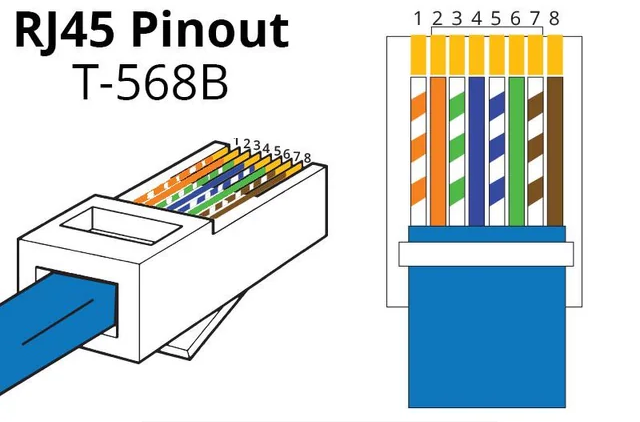
\includegraphics[width=0.4\linewidth]{./images/RJ45.png}
\end{figure}

\begin{table}[htp]
	\centering
	\begin{tabular}{|c|c|c|c|}
		\hline
		Pin & Colore & Polarità & Utilizzo\\
		\hline
		1 & bianco/arancione & + & Trasmissione (Tx)\\
		2 & arancione & - & Trasmissione (Tx)\\
		3 & bianco/verde & + & Ricezione dati (Rx)\\
		4 & blu & - & Bidirezionale dati (Bi3)\\
		5 & bianco/blu & + & Bidirezionale dati (Bi3)\\
		6 & verde & - & Ricezione dati (Rx)\\
		7 & bianco/marrone & + & Bidirezionale dati (Bi4)\\
		8 & marrone & - & Bidirezionale dati (Bi4)\\
		\hline
	\end{tabular}
\end{table}

La polarità opposta nei segnali trasmessi nei cavi twisted pair permette di ridurre il rumore con estrema facilità.
Supponiamo che un bit venga trasmesso a 1V in due coppie di cavi con polarità opposta ($A: +1V$,  $B: -1V$). Nei sistemi \textbf{differenziali}, il segnale sta nella differenza tra le coppie di segnali, e quindi:
$$
1 V - (-1V) = 1V+1V = 2V
$$

Supponiamo adesso di indurre un rumore di $+0.5V$ al nostro cavo (e quindi su entrambi i cavi della coppia). 

$$
(1V+0.5V) - (0.5V-1V) = 1.5V - (-0.5V)=1.5V+0.5V = 2V
$$

\begin{figure}[htp]
	\centering
	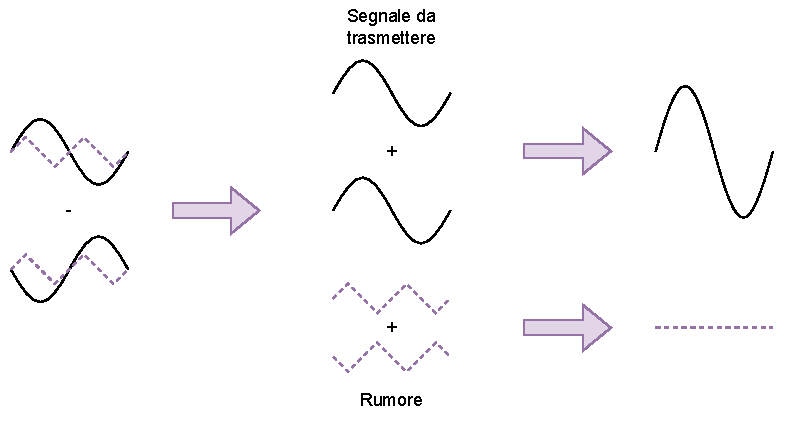
\includegraphics[width=0.85\linewidth]{./images/noise canceling (1).pdf}
	\caption{Esempio di cancellazione del rumore}
\end{figure}

\newpage

\subsubsection{Distinzione: cavi diretti e cavi incrociati}
\begin{itemize}
	\item \textbf{Cavo incrociato.}\\
	La disposizione dei doppini è diversa tra le due estremità. È usato per collegare dispositivi simili (router a router).
	\item \textbf{Cavo diretto.}\\
	La disposizione dei doppini è uguale tra le due estremità. È usato per collegare dispositivi diversi (pc a router).
\end{itemize}
\section{Frame Ethernet}
\begin{figure}[htp]
	\centering
	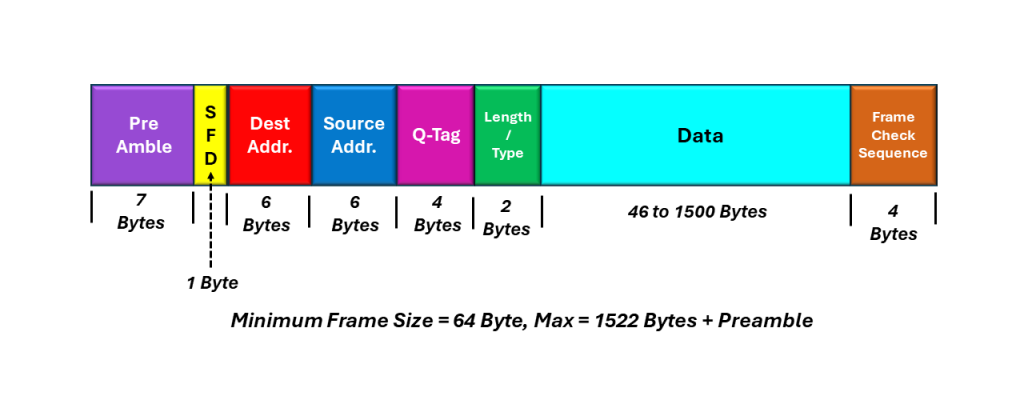
\includegraphics[width=1\linewidth]{./images/frameethernet.png}
\end{figure}
\begin{itemize}
	\item \textbf{Preambolo}.\\
	7 byte a \verb|10101010| per sincronizzare i clock delle schede di rete.
	\item \textbf{Start Frame Delimiter}.\\
	Un byte a \verb|10101011| per interrompere il pattern del preambolo e indicare l'inizio del frame.
	\item \textbf{MAC address destinatario}.\\
	6 byte.
	\item \textbf{MAC address mittente}.\\
	6 byte.
	\item \textbf{Q-Tag/VLAN Tag}.\\
	È il tag presente \textbf{esclusivamente nei frame Ethernet che supportano le VLAN}. Non è sempre presente, in quanto non tutti i frame Ethernet sono \textit{tagged}. 4 byte.
	\item \textbf{Type/length}.\\
	2 byte che identificano il tipo di connessione (EtherType, IPv4, IPv6, ARP,$\dots$), se ha valore superiore a 1500, altrimenti, la lunghezza del data field.
	\item \textbf{Data field}.\\
	Minimo 46 byte, massimo 1500 byte. Se il frame da inviare non supera la dimensione minima, si usa un \textbf{padding}. Se il frame supera la dimensione massima, si frammenta.
	\item \textbf{Frame check sequence}.\\
	4 byte dedicati al controllo CRC per rilevare (e/o correggere) errori.
\end{itemize}

\newpage

\subsection{Codifica di Manchester}
È una codifica che nasce per ovviare ad alcune delle criticità relative alla trasmissione che già conosciamo:
\begin{itemize}
	\item \textbf{Ambiguità delle lunghe sequenze.}\\
	La codifica di Manchester forza delle transizioni obbligatorie quando trasmette dei bit. Diventa più facile riconoscere malfunzionamenti e interruzioni della trasmissione.
	\item \textbf{Sincronizzazione precaria.}\\
	Ogni bit contiene al suo interno una transizione. Non può perdersi la sincronizzazione.
\end{itemize}

Viene realizzata tramite un'operazione di $XOR$ tra il segnale di clock e il segnale dati. Ogni bit è codificato come un fronte di salita (1) o un fronte di discesa (0). In questo modo, il \textit{bitstream} e il segnale di clock sono, in un certo senso, trasmessi contemporaneamente.

\begin{figure}[htp]
	\centering
	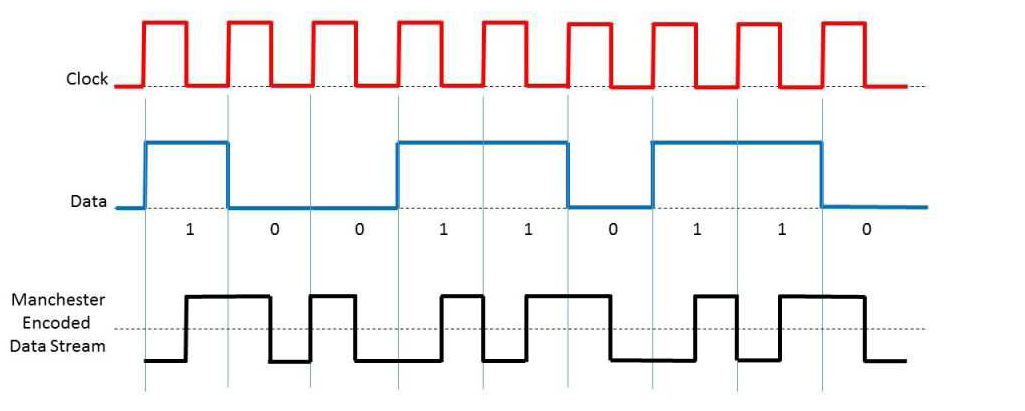
\includegraphics[width=1\linewidth]{./images/manchesterencoding1.png}
\end{figure}

Tuttavia, questa codifica è influenzata dalla polarità del segnale trasmesso. Se il segnale codificato viene invertito, bisogna invertire anche la sua codifica. Possiamo risolvere il problema usando la codifica di Manchester differenziale.


\subsubsection{Codifica di Manchester differenziale}
Rende la codifica di Manchester insensibile alla polarità. Ogni bit presenta almeno una transizione a metà periodo di clock. Il valore del bit dipenderà dalla presenza o meno di una transizione (in particolare, fronte di salita) all'inizio del periodo di clock.
\begin{itemize}
	\item Bit 0: transizione.
	\item Bit 1: assenza di transizione.
\end{itemize}

\begin{figure}[htp]
	\centering
	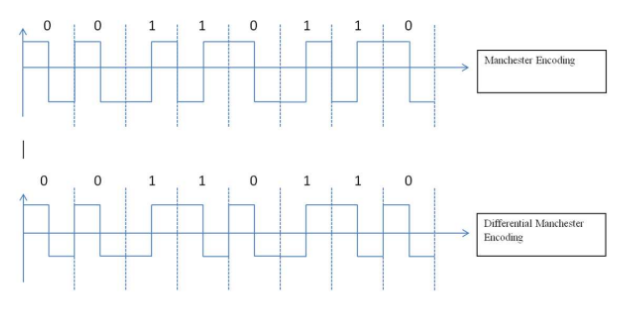
\includegraphics[width=0.8\linewidth]{./images/Manchester.png}
	\caption{Codifiche di Manchester a confronto}
\end{figure}

\newpage

\section{Gigabit Ethernet}
È lo standard Ethernet che raggiunge i 1000Mbps, ovvero 1Gbps. Andiamo a scomporre come le scelte prese permettano di raggiungere queste velocità.
\begin{enumerate}
	\item \textbf{Rimossa la codifica 4B5B.}\\
	$100 \to 125$ Mbps. Rimuoviamo l'overhead del $25\%$ della codifica 4B5B. La sincronizzazione è garantita dalla codifica di Manchester.
	
	\item \textbf{4 doppini di rame usati allo stesso tempo}.\\
	$125 \to 4\cdot125 = 500$ Mbps.
	
	\item \textbf{Trasmissione full-duplex}.\\
	$500$ Mbps full-duplex.
	
	\item \textbf{5 livelli per baud invece di 3}.\\
	5 livelli su ogni canale di trasmissione. Con 4 canali, otteniamo $5^4=625$ combinazioni, e quindi $\log_2(625) \approx 9$ bit
	
	\item \textbf{Trasmissione finale:} Con $10^6$ frequenza di simbolo $125 \cdot 10^6 \cdot 9$bit = 1 Gbit lordo.
	
	\item \textbf{Forward Error Correction}.
\end{enumerate}

\subsection{Filtro DuoBinary}
Il seguente filtro, detto DuoBinary, si occupa della codifica.
\begin{figure}[htp]
	\centering
	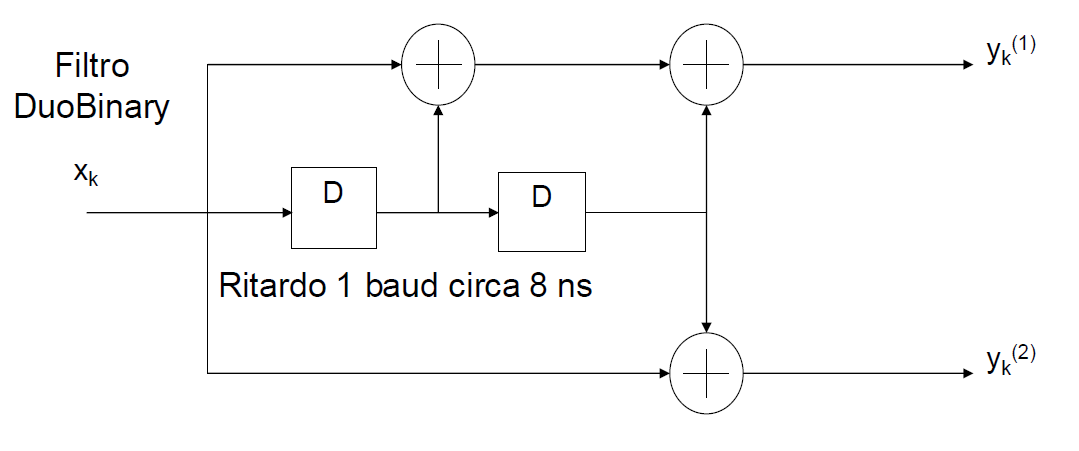
\includegraphics[width=0.75\linewidth]{./images/duobinary.png}
\end{figure}

\begin{enumerate}
	\item Il bit in entrata viene sdoppiato in due segnali.
	\item Introduce un ritardo ad uno dei due segnali.
	\item Si stringe lo spettro del segnale: \textbf{un simbolo viene codificato in due simboli}.
\end{enumerate}

\newpage

\subsection{Decodifica 4D}
La decodifica 4D, detta di Viterbi, viene eseguita tramite un automa a stati finiti.

\begin{figure}[htp]
	\centering
	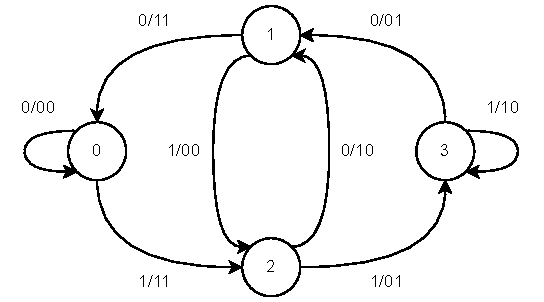
\includegraphics[width=0.75\linewidth]{./images/trellis.drawio.pdf}
\end{figure}

Ciò che viene fatto è una \textbf{Trellis code modulation}. Raddoppiando il numero di bit per rappresentare un bit d'informazione, gli errori peseranno meno sull'informazione complessiva. Tuttavia è grazie alle transizioni dell'automa limitate che è possibile capire quando è avvenuto un errore: la distanza di Hamming delle stringhe possibili valutate rispetto a quella consegnata, ci permette di stabilire come effettuare la correzione.

\newpage

\section{Strutture Ethernet}
Hub e bridge sono strutture fisiche che permettono di collegare le varie sottoreti. Sono strutture molto diverse, e al giorno d'oggi l'hub è obsoleto. Il bridge è alla base di tutti gli switch moderni.

\subsection{Differenze tra hub e bridge}
L'ormai obsoleto hub:
\begin{itemize}
	\item Lavora principalmente al livello fisico.
	\item Ripete e rigenera il segnale su tutte le porte.
	\item Il dominio di collisione tra tutti i dispositivi collegati è unico.
	\item Broadcast domain unico. 
\end{itemize}
Il bridge, invece:
\begin{itemize}
	\item Lavora a livello data link.
	\item Filtra e inoltra in base all'indirizzo MAC 
	\item Nel bridge ogni porta crea (idealmente) un dominio di collisione separato.
	\item Broadcast domain unico.
\end{itemize}

\subsection{Switch}
È un dispositivo che trasmette pacchetti ricevuti a uno o più dispositivi destinatari. È più espandibile in termini di numero di porte, rispetto al bridge, ed effettua operazioni di \textbf{inoltro} (individuare a quale interfaccia mandare il frame) e \textbf{filtraggio} (capire quando scartare un frame). Uno switch contiene al suo interno una \textbf{switch table} con record del tipo \verb|Indirizzo MAC - Interfaccia - Tempo|.
Il tempo viene utilizzato per stabilire quando un dispositivo non è più presente nella rete: verrà dedotto in quanto non verranno mandati più pacchetti al suo indirizzo MAC per molto tempo. Gli switch sono full duplex, senza collisioni.

\newpage


\section{VLAN}
Le LAN virtuali permettono di creare delle LAN logiche indipendenti sulla stessa struttura fisica. 

\begin{figure}[htp]
	\centering
	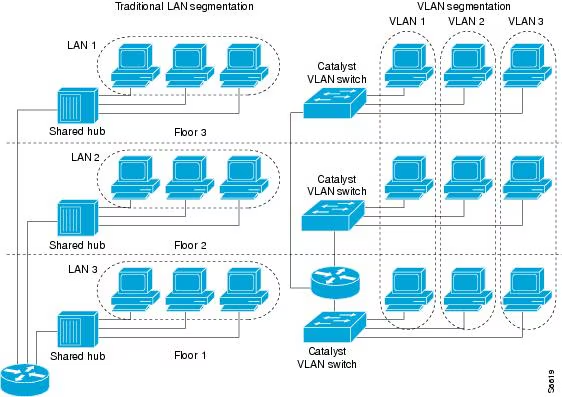
\includegraphics[width=0.75\linewidth]{./images/vlan.png}
\end{figure}

Permette di risparmiare su costi, sulla manodopera e sulla complessità dietro il ricablaggio di una rete, per modificarne la struttura logica. Sono quindi delle vere e proprie LAN logiche separate che risiedono sopra la struttura fisica. Le LAN virtuali rimappano le tabelle di forward del bridge senza modificare la cablatura. Una porta può essere associata a una e una sola VLAN, altrimenti si riscontrerebbero collisioni.

\subsection{Scopo delle VLAN}
\begin{itemize}
	\item \textbf{Riutilizzo dell'architettura di partenza} con conseguente risparmio.
	\item \textbf{Flessibilità}.\\
	Molto più facile spostare gli utenti tra le VLAN.
	\item \textbf{Prestazioni migliori}.\\
	Isolando il broadcasting nelle VLAN,
	\item \textbf{Sicurezza}.\\
	È semplice isolare dei sistemi tramite le VLAN.
\end{itemize}

\subsection{VLAN basata su porte}
Lo switch può essere \textbf{partizionato logicamente} in più insiemi di porte. Le porte possono essere associate a delle VLAN. Nell'header dei frame DLL è presente un identificatore di VLAN.

\begin{itemize}
	\item \textbf{Tag Protocol Identifier.}\\
	16 bit.
	\item \textbf{Priority.}\\
	Identifica il livello di priorità. 3 bit.
	\item \textbf{Canonical Format Identifier.}\\
	1 bit che specifica se il frame è untagged. Il flag a 0 indica che il meccanismo di VLAN non è supportato.
	\item \textbf{Virtual Lan Identifier.}\\
	12 bit.
\end{itemize}



\newpage

\subsection{LAN vs Dispositivi Legacy}
I dispositivi legacy che non supportano le VLAN, ignorano tutti i frame tagged VLAN a loro in arrivo.

\begin{figure}[htp]
	\centering
	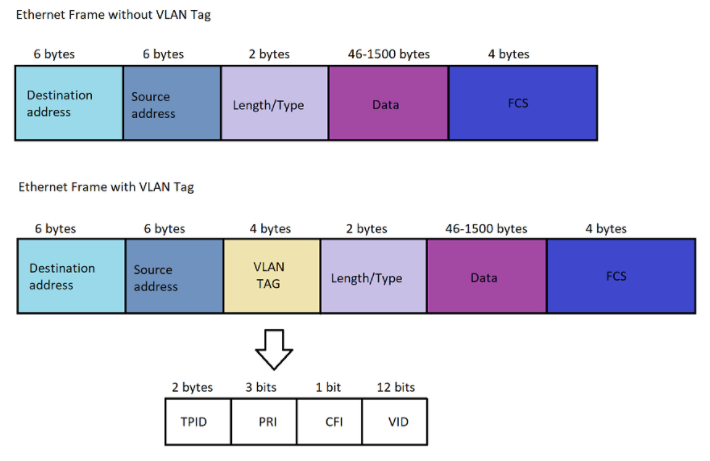
\includegraphics[width=0.75\linewidth]{./images/vlanvslegacy.png}
\end{figure}

\begin{figure}[htp]
	\centering
	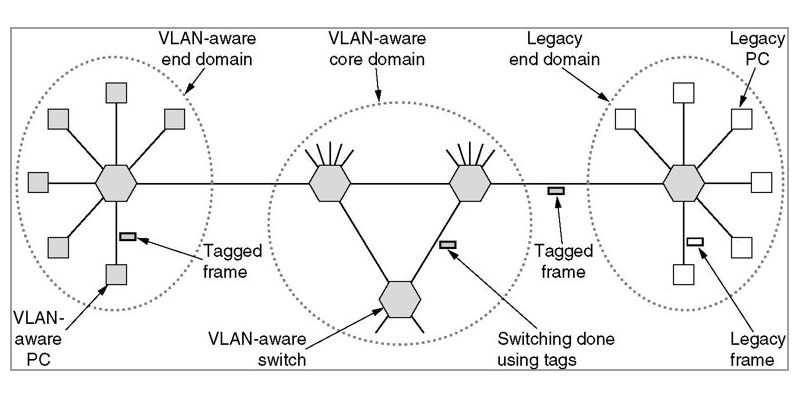
\includegraphics[width=1\linewidth]{./images/VLAN3.png}
	\caption{Una rete con dispositivi VLAN e legacy}
\end{figure}
